\documentclass[times, utf8, seminar, numeric]{fer}
\usepackage{booktabs, url, hyperref}
\usepackage{verbatim}
\usepackage{moreverb}
\usepackage{subfigure}
\usepackage{caption}
\usepackage{epstopdf}

\hypersetup{
   colorlinks,
   citecolor=black,
   filecolor=black,
   linkcolor=black,
   urlcolor=black
}

%dodatak za programski kod
\usepackage{listings}
\usepackage{color}
\usepackage{setspace}
\definecolor{dkgreen}{rgb}{0,0.6,0}
\definecolor{gray}{rgb}{0.5,0.5,0.5}
\definecolor{mauve}{rgb}{0.58,0,0.82}

\lstset{frame=tb,
  language=Java,
  aboveskip=3mm,
  belowskip=3mm,
  showstringspaces=false,
  columns=flexible,
  basicstyle={\small\ttfamily},
  numbers=left,
  numberstyle=\small\color{gray},
  keywordstyle=\color{blue},
  commentstyle=\color{dkgreen},
  stringstyle=\color{mauve},
  breaklines=true,
  breakatwhitespace=true,
  tabsize=2
}


\begin{document}

\nocite{saitou}\nocite{phylpro}\nocite{wiki}\nocite{mbt}

% TODO: Navedite naslov rada.
\title{Algoritam "Neighbor joining"}

% TODO: Navedite vaše ime i prezime.
\author{\itshape{Filip Beć}\\
				 \itshape{Zorana Ćurković}\\
				 \itshape{Goran Gašić}\\
				 \itshape{Melita Kokot}\\
				 \itshape{Dino Šantl}\\
				 \itshape{Igor Smolkovič}
				 }

% TODO: Navedite ime i prezime mentora.
\voditelj{\itshape{Dr. sc. Mirjana Domazet-Lošo}\\ \itshape{Doc. dr. sc. Mile Šikić}}

\maketitle

\tableofcontents

\chapter{Opis algoritma}

Algoritam \emph{Neighbor joining} služi za izgradnju filogenetskog stabla. Ulaz algoritma su evolucijske udaljenosti (matrica udaljenosti čvorova). Izlaz algoritma je stablo s težinskim bridovima. Cilj algoritma izgraditi je minimalno razapinjajuće filogenetsko stablo. Algoritam nužno ne pronalazi takvo stablo ali rješenja su često minimalna razapinjajuća filogenetska stabla ili blizu toga \cite{saitou}. Glavni razlog je smanjenje vremenske složenosti, jer u praksi nije izvedivo ispitivanje svih mogućih stabala. Stablo se gradi od dna prema vrhu. Algoritam je pohlepan jer za jednom sparene čvorove ne ispituje točnost tog koraka.

Algoritam se sastoji od dva dijela: uparivanje čvorova i završni korak. Algoritam kreće od matrice udaljenosti nad kojom zaključuje koja dva čvora je potrebno upariti. Kada su poznata dva čvora koja se trebaju upariti, stvara se novi čvor koji se spaja s dva odabrana. Dva odabrana čvora se brišu iz matrice udaljenosti, a novi čvor se ubaci u matricu udaljenosti. Taj postupak se izvršava $N-3$ puta, gdje je $N$ početni broj čvorova. Završni korak uzima zadnja tri čvora koja su ostala u matrici udaljenosti, stvara novi čvor i spaja novi čvor s tri zadnja čvora u matrici udaljenosti. Formalno algoritam izgleda ovako:
\begin{enumerate}
	\item \textbf{Ulaz}: matrica udaljenosti
	\item Na temelju trenutne matrice udaljenosti izračunaj matricu \textbf{Q}
	\item U matrici \textbf{Q} pronađi najmanju vrijednost $Q(i,j)$ i pripadajuće čvorove $(i,j)$.
	\item Stvori novi čvor $w$ i dva nova brida: $(w,i)$ i $(w,j)$ te izračunaj udaljenosti $d(w,i)$ i $d(w,j)$ i zapiši ih na pripadajući brid.
	\item Iz matrice udaljenosti izbriši čvorove $i$ i $j$, te dodaj u matricu novi čvor $w$ - potrebno je izračunati udaljenosti do novoga čvora $w$
	\item Ako postoji više od 3 čvora u matrici udaljenosti skoči na korak 2.
	\item Stvori novi čvor $w$ i napravi 3 brida s preostalim čvorovima u matrici udaljenosti te izračunaj i pridruži vrijednost bridovima 
\end{enumerate}

\section{Matrica Q}
Matrica \textbf{Q} pomoćna je matrica iz koje se određuje par čvorova koji će biti susjedni. Matrica \textbf{Q} kao kriterij uzima osim udaljenosti čvorova $i$ i $j$ utjecaj njihovih susjeda. Dokaz da je najmanja vrijednost matrice \textbf{Q} pripada susjednim čvorovima dan je u \cite{saitou}. Matrica \textbf{Q} izračunava se na sljedeći način:

\begin{equation}
	Q(i,j) = (r-2) d(i,j) - \sum_{k=1}^{r}d(i,k) - \sum_{k=1}^{r}d(j,k)
\end{equation}
, gdje su $i$, $j$ indeksi čvorova, r je trenutni broj čvorova u matrici udaljenosti. Oznake $d(i,j)$, $d(i,k)$ i $d(j,k)$ predstavljaju vrijednosti u matrici udaljenosti. Čvorovi $i$ i $j$ moraju biti različiti.

\section{Računanje vrijednosti bridova}

Nakon što se stvore novi bridovi u stablu potrebno je odrediti njihovu vrijednost. U svakom koraku uparivanja stvore se dva nova brida. U završnom koraku stvore se tri nova brida.

Nakon što se čvorovi $i$ i $j$ proglase susjednima stvara se novi čvor $w$. Potrebno je odrediti udaljenosti $d(i, w)$ i $d(j,w)$. Udaljenosti se određuju prema formulama:

\begin{equation}
d(i,w) = \frac{1}{2}d(i,j)+\frac{1}{2(r-2)} \left [ \sum_{k=1}^{r}d(i,k) - \sum_{k=1}^{r}d(j,k) \right ]
\end{equation}
, gdje je $r$ trenutni broj čvorova u matrici udaljenosti.

Kako vrijedi $d(i,j)=d(i,w)+d(j,w)$, iz toga sljedi:
\begin{equation}
d(j,w) = d(i,j) - d(i,w)
\end{equation}

\section{Računanje udaljenosti do novog čvora}

Pri ubacivanju novog čvora u matricu udaljenosti potrebno je izračunati udaljenost od svih starih čvorova do novog čvora $w$. Udaljenost se računa prema formuli: 

\begin{equation}
d(k,w) = \frac{1}{2} \left [ d(i,k) + d(j,k) - d(i,j) \right ]
\end{equation}
, gdje je $k$ bilo koji stari čvor u matrici udaljenosti. Čvorovi $i$ i $j$ su upravo spojeni čvorovi. 

\section{Složenost algoritma}

Algoritam mora izvršiti korak uparivanja $N-3$ puta, gdje je $N$ broj čvorova u početnoj matrici udaljenosti. U svakom koraku potrebno je izračunati matricu \textbf{Q} koja je dimenzije $r\times r$, gdje je $r$ trenutni broj čvorova. Ako se predprocesiraju sume u prije navedenim formulama u $O(N)$ vremenu, tada za računanje matrice \textbf{Q} potrebno $O(N^2)$ vremena. Zbog toga je ukupna vremenska složenost algritma $O(N^3)$. Memorijska složenost je $O(N^2)$ jer se pamti matrica udaljenosti.

\chapter{Primjer izvođenja}

Raspolažemo skupom od $5$ taksona $(\textup{Dog},\textup{Cat},\textup{Rabbit},\textup{Monkey},\textup{Cow})$ te pridanim udaljenostima među njima definiranim matricom udaljenosti:
\begin{table}[h]
	\centering
    \begin{tabular}{|l|l|l|l|l|l|}
    \hline
    ~ & Dog  & Cat  & Rabbit  & Duck  & Swan  \\ \hline
    Dog & 0  & 5  & 17 & 15 & 13 \\ \hline
    Cat & 5  & 0  & 9  & 19 & 14 \\ \hline
    Rabbit & 17 & 9  & 0  & 20 & 16 \\ \hline
    Duck & 15 & 19 & 20 & 0  & 12 \\ \hline
    Swan & 13 & 14 & 16 & 12 & 0  \\ \hline
    \end{tabular}
\end{table}

Algoritam će biti proveden u $N-3=2$ koraka. \newline

\begin{figure}[htb]
\centering
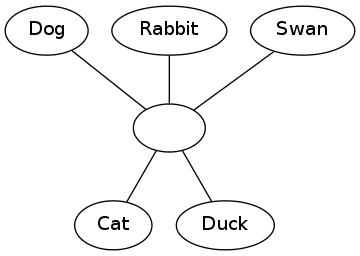
\includegraphics[scale=0.6]{./img/pocetni.png}
\caption{Početno stablo}
\end{figure}

\newpage
\section{1. korak}
Izračunamo matricu $Q$ te tražimo par $(i,j)$ koji ima najmanju vrijednost:

\begin{table}[h]
	\centering
    \begin{tabular}{|l|l|l|l|l|l|}
    \hline
    ~ & Dog  & Cat  & Rabbit  & Duck  & Swan  \\ \hline
    Dog & 0   & -82 & -61 & -71 & -66 \\ \hline
    Cat & -82 & 0   & -82 & -56 & -60 \\ \hline
    Rabbit & -61 & -82 & 0   & -68 & -69 \\ \hline
    Duck & -71 & -56 & -68 & 0   & \textbf{-85} \\ \hline
    Swan & -66 & -60 & -69 & -85 & 0   \\ \hline
    \end{tabular}
\end{table}

$i = \textup{Duck}, j = \textup{Swan}, Q_{min} = -85$. Taksone Duck i Swan spajamo u novi čvor $\textup{node1}$ te računamo udaljenosti: 

\indent $d(\textup{Duck},\textup{node1}) = 7.833$, \newline
\indent $d(\textup{Swan},\textup{node1}) = 4.166$


Preostale udaljenosti $d(k,\textup{node1})$ definirane su novom matricom udaljenosti :

\begin{table}[h]
	\centering
    \begin{tabular}{|l|l|l|l|l|l|}
    \hline
	~ & Dog  & Cat    & Rabbit  & node1 \\ \hline
    Dog     & 0  & 5    & 17 & 8     \\ \hline
    Cat   & 5  & 0    & 9  & 10.5  \\ \hline
    Rabbit     & 17 & 9    & 0  & 12    \\ \hline
    node1 & 8  & 10.5 & 12 & 0     \\ \hline
    \end{tabular}
\end{table}

\begin{figure}[htb]
\centering
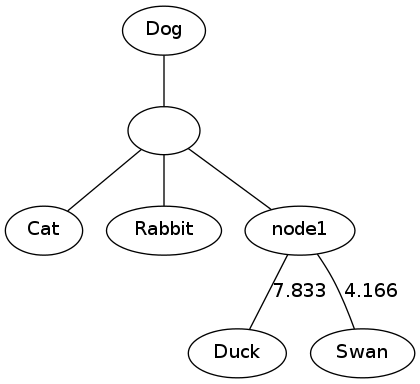
\includegraphics[scale=0.6]{./img/prvi.png}
\caption{Trenutno stablo}
\end{figure}

\newpage
\section{2. korak}
Izračunamo matricu $Q$ te tražimo par $(i,j)$ koji ima najmanju vrijednost:

\begin{table}[h]
	\centering
    \begin{tabular}{|l|l|l|l|l|l|}
    \hline
~     & Dog     & Cat     & Rabbit     & node1 \\ \hline
    Dog     & 0     & \textbf{-44.5} & -34   & -44.5 \\ \hline
    Cat     & -44.5 & 0     & -44.5 & -34   \\ \hline
    Rabbit     & -34   & -44.5 & 0     & -44.5 \\ \hline
    node1 & -44.5 & -34   & -44.5 & 0     \\ \hline
    \end{tabular}
\end{table}

$i = \textup{Dog}, j = \textup{Cat}, Q_{min} = -44.5$. Taksone Dog i Cat spajamo u novi čvor $\textup{node2}$ te računamo udaljenosti: 

\indent $d(\textup{Dog},\textup{node2}) = 3.875$, \newline
\indent $d(\textup{Cat},\textup{node2}) = 1.125$ \newline


Preostale udaljenosti $d(k,\textup{node2})$ definirane su novom matricom udaljenosti :

\begin{table}[h]
	\centering
    \begin{tabular}{|l|l|l|l|}
    \hline
    ~     & node2 & Rabbit    & node1 \\ \hline
    node2 & 0     & 10.5 & 6.75  \\ \hline
    Rabbit     & 10.5  & 0    & 12    \\ \hline
    node1 & 6.75  & 12   & 0     \\ \hline
    \end{tabular}
\end{table}

Potrebno je još spojiti preostala $3$ čvora. U svrhu spajanja stvaramo novi čvor node3. Poznate su nam udaljenosti $d(\textup{node2},\textup{Rabbit})$, $d(\textup{node2}, \textup{node1})$ i  $d(\textup{Rabbit},\textup{node1})$. Temeljem tih udaljenosti možemo izračunati posljednja tri luka. \newline

\indent $d(\textup{node3}, \textup{node2}) = 0.5 * (d(\textup{node2}, \textup{node1}) + d(\textup{node2}, \textup{Rabbit}) - d(\textup{node1}, \textup{Rabbit})) $ \newline
\indent $= 2.625$ \newline

\indent $d(\textup{node3},\textup{ node1}) = 0.5 * (d(\textup{node1}, \textup{Rabbit}) + d(\textup{node2}, \textup{Rabbit}) - d(\textup{node1}, \textup{node2})) $ \newline
\indent $=4.125 $ \newline

\indent $d(\textup{node3},\textup{Rabbit}) = 0.5 * (d(\textup{node1}, \textup{Rabbit}) + d(\textup{node1}, \textup{node2}) - d(\textup{node2}, \textup{Rabbit})) $ \newline
\indent = 7.875 \newline


\begin{figure}[htb]
\centering
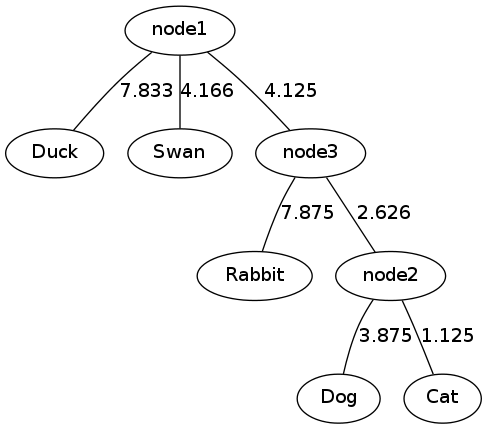
\includegraphics[scale=0.6]{./img/zadnji.png}
\caption{Konačno stablo}
\end{figure}

\chapter{Testiranje i usporedbe}

\chapter{Zaključak}

\bibliography{literatura}
%\bibliographystyle{fer} %promijena za citiranje po redu ieeetr
\bibliographystyle{ieeetr}

\begin{comment}
\begin{sazetak}
Simbolička regresija je postupak otkrivanja matematičkog izraza u skupu podataka. Daje se pregled metoda za simboličku regresiju s naglaskom na genetsko programiranje. Obrađuju se problemi kao što su domene funkcija (nisu definirane na cijelom skupu realnih brojeva). Problemi se rješavaju intervalnom aritmetikom i linearnim skaliranjem. Na kraju se ukratko opisuje mogućnost paralelizacije i primjene. 

\kljucnerijeci{genetsko programiranje, s}

\end{sazetak}

% TODO: Navedite naslov na engleskom jeziku.
\engtitle{Application of graphics coprocessors for program execution on stream programming model}

\begin{abstract}


\keywords{GPU, StreamIt, Sponge, StreamGate, CUDA, stream model, filter, optimization, graphics card}
\end{abstract}
\end{comment}

\end{document}
